% Options for packages loaded elsewhere
\PassOptionsToPackage{unicode}{hyperref}
\PassOptionsToPackage{hyphens}{url}
%
\documentclass[
  english,
  ,jou, a4paper,floatsintext]{apa6}
\usepackage{lmodern}
\usepackage{amssymb,amsmath}
\usepackage{ifxetex,ifluatex}
\ifnum 0\ifxetex 1\fi\ifluatex 1\fi=0 % if pdftex
  \usepackage[T1]{fontenc}
  \usepackage[utf8]{inputenc}
  \usepackage{textcomp} % provide euro and other symbols
\else % if luatex or xetex
  \usepackage{unicode-math}
  \defaultfontfeatures{Scale=MatchLowercase}
  \defaultfontfeatures[\rmfamily]{Ligatures=TeX,Scale=1}
\fi
% Use upquote if available, for straight quotes in verbatim environments
\IfFileExists{upquote.sty}{\usepackage{upquote}}{}
\IfFileExists{microtype.sty}{% use microtype if available
  \usepackage[]{microtype}
  \UseMicrotypeSet[protrusion]{basicmath} % disable protrusion for tt fonts
}{}
\makeatletter
\@ifundefined{KOMAClassName}{% if non-KOMA class
  \IfFileExists{parskip.sty}{%
    \usepackage{parskip}
  }{% else
    \setlength{\parindent}{0pt}
    \setlength{\parskip}{6pt plus 2pt minus 1pt}}
}{% if KOMA class
  \KOMAoptions{parskip=half}}
\makeatother
\usepackage{xcolor}
\IfFileExists{xurl.sty}{\usepackage{xurl}}{} % add URL line breaks if available
\IfFileExists{bookmark.sty}{\usepackage{bookmark}}{\usepackage{hyperref}}
\hypersetup{
  pdftitle={Reviewers' Decision to Sign Reviews is Related to Their Recommendation},
  pdflang={en-EN},
  pdfkeywords={Peer Review, Open Reviews, Transparency, Open Science},
  hidelinks,
  pdfcreator={LaTeX via pandoc}}
\urlstyle{same} % disable monospaced font for URLs
\usepackage{graphicx,grffile}
\makeatletter
\def\maxwidth{\ifdim\Gin@nat@width>\linewidth\linewidth\else\Gin@nat@width\fi}
\def\maxheight{\ifdim\Gin@nat@height>\textheight\textheight\else\Gin@nat@height\fi}
\makeatother
% Scale images if necessary, so that they will not overflow the page
% margins by default, and it is still possible to overwrite the defaults
% using explicit options in \includegraphics[width, height, ...]{}
\setkeys{Gin}{width=\maxwidth,height=\maxheight,keepaspectratio}
% Set default figure placement to htbp
\makeatletter
\def\fps@figure{htbp}
\makeatother
\setlength{\emergencystretch}{3em} % prevent overfull lines
\providecommand{\tightlist}{%
  \setlength{\itemsep}{0pt}\setlength{\parskip}{0pt}}
\setcounter{secnumdepth}{-\maxdimen} % remove section numbering
% Make \paragraph and \subparagraph free-standing
\ifx\paragraph\undefined\else
  \let\oldparagraph\paragraph
  \renewcommand{\paragraph}[1]{\oldparagraph{#1}\mbox{}}
\fi
\ifx\subparagraph\undefined\else
  \let\oldsubparagraph\subparagraph
  \renewcommand{\subparagraph}[1]{\oldsubparagraph{#1}\mbox{}}
\fi
% Manuscript styling
\usepackage{upgreek}
\captionsetup{font=singlespacing,justification=justified}

% Table formatting
\usepackage{longtable}
\usepackage{lscape}
% \usepackage[counterclockwise]{rotating}   % Landscape page setup for large tables
\usepackage{multirow}		% Table styling
\usepackage{tabularx}		% Control Column width
\usepackage[flushleft]{threeparttable}	% Allows for three part tables with a specified notes section
\usepackage{threeparttablex}            % Lets threeparttable work with longtable

% Create new environments so endfloat can handle them
% \newenvironment{ltable}
%   {\begin{landscape}\begin{center}\begin{threeparttable}}
%   {\end{threeparttable}\end{center}\end{landscape}}
\newenvironment{lltable}{\begin{landscape}\begin{center}\begin{ThreePartTable}}{\end{ThreePartTable}\end{center}\end{landscape}}

% Enables adjusting longtable caption width to table width
% Solution found at http://golatex.de/longtable-mit-caption-so-breit-wie-die-tabelle-t15767.html
\makeatletter
\newcommand\LastLTentrywidth{1em}
\newlength\longtablewidth
\setlength{\longtablewidth}{1in}
\newcommand{\getlongtablewidth}{\begingroup \ifcsname LT@\roman{LT@tables}\endcsname \global\longtablewidth=0pt \renewcommand{\LT@entry}[2]{\global\advance\longtablewidth by ##2\relax\gdef\LastLTentrywidth{##2}}\@nameuse{LT@\roman{LT@tables}} \fi \endgroup}

% \setlength{\parindent}{0.5in}
% \setlength{\parskip}{0pt plus 0pt minus 0pt}

% \usepackage{etoolbox}
\makeatletter
\patchcmd{\HyOrg@maketitle}
  {\section{\normalfont\normalsize\abstractname}}
  {\section*{\normalfont\normalsize\abstractname}}
  {}{\typeout{Failed to patch abstract.}}
\makeatother
\shorttitle{Signing Open Reviews}
\author{Nino van Sambeek\textsuperscript{1}\ \& Daniel Lakens\textsuperscript{1}}
\affiliation{
\vspace{0.5cm}
\textsuperscript{1} Eindhoven University of Technology, The Netherlands}
\authornote{Submitted to Meta-Psychology. Click here to follow the fully transparent editorial process of this submission. Participate in open peer review by commenting through hypothes.is directly on this preprint. This work was supported by the Netherlands Organization for Scientific Research (NWO) VIDI grant 452-17-013. All data underlying this reproducible manuscript are available at https://osf.io/9526a/


Correspondence concerning this article should be addressed to Daniel Lakens, ATLAS 9.402, 5600 MB, Eindhoven, The Netherlands. E-mail: D.Lakens@tue.nl}
\keywords{Peer Review, Open Reviews, Transparency, Open Science\newline\indent Word count: 2711}
\usepackage{dblfloatfix}


\usepackage{csquotes}
\ifxetex
  % Load polyglossia as late as possible: uses bidi with RTL langages (e.g. Hebrew, Arabic)
  \usepackage{polyglossia}
  \setmainlanguage[]{english}
\else
  \usepackage[shorthands=off,main=english]{babel}
\fi

\title{Reviewers' Decision to Sign Reviews is Related to Their Recommendation}

\date{}

\abstract{
Surveys indicate that researchers generally have a positive attitude towards open peer review when this consists of making reviews available alongside published articles. Researchers are more negative about revealing the identity of reviewers. They worry reviewers will be less likely to express criticism if their identity is known to authors. Experiments suggest that reviewers are somewhat less likely to recommend rejection when they are told their identity will be communicated to authors, than when they will remain anonymous. One recent study revealed reviewers in five journals who voluntarily signed their reviews gave more positive recommendations than those who did not sign their reviews. We replicate and extend this finding by analyzing 12010 open reviews in PeerJ and 4188 reviews in the Royal Society Open Science where authors can voluntarily sign their reviews. These results based on behavioral data from real peer reviews across a wide range of scientific disciplines demonstrate convincingly that reviewers' decision to sign is related to their recommendation. The proportion of signed reviews was higher for more positive recommendations, than for more negative recommendations. We also share all 23649 text mined reviews as raw data underlying our results that can be re-used by researchers interested in peer review.
}

\begin{document}
\maketitle

As technology advances, science advances. The rise of the internet has made it possible to transparently share all steps in the scientific process (Spellman, 2015). This includes opening up the peer review process. An increasing number of journals have started to make peer review reports available alongside published articles as part of ongoing experiments that aim to improve peer review (Bruce, Chauvin, Trinquart, Ravaud, \& Boutron, 2016). Open peer review can be implemented by making peer reviews available, but also by revealing the identity of reviewers during or after the peer review process. An important argument in favour of revealing the identity of reviewers is that they can receive credit for their work (Godlee, 2002). However, scientists do not feel these benefits outweigh possible costs, and are worried that criticism on manuscripts might lead to backlash from the authors in the future. Some reviewers might accept these negative consequences, while other might choose to strategically reveal their identity only for positive reviews they write.

Researchers self-report that they would be less likely to review for a journal if their identity is made public, and anecdotally mention that signed reviews would make it more difficult to be honest about manuscripts they believe are poor quality (Mulligan, Hall, \& Raphael, 2013). A more recent survey found that 50.8\% of almost 3000 scientists believe that revealing the identity of reviewers would make peer review worse (Ross-Hellauer, Deppe, \& Schmidt, 2017). Almost two-thirds of respondents believed reviewers would be less likely to deliver strong criticisms if their identity became known to the authors.

These self-report studies are complemented by experiments in which reviewers are randomly assigned to a condition where their identity would be revealed during the peer review process (Walsh, Rooney, Appleby, \& Wilkinson, 2000). Reviewers in the condition where their identity was revealed were less likely to recommend rejection (n = 30) than reviewers who remained anonymous (n = 51). This suggests that a causal effect exists between knowing your identity will be revealed, and the recommendation that is made during the peer review process. Based on a small-scale meta-analysis of four studies Bruce and colleagues (2016) found support for the conclusion that reviewers are somewhat less likely to recommend rejection when they have to sign their reviews.

Although the self-report studies and the experiments clearly suggest that reviewers worry about having their name attached to more critical reviews they write, so far little is known about what reviewers actually do when given the opportunity to sign their reviews. The trade-off between the benefit of getting credit when performing peer reviews and the risk of negative consequences when signing critical reviews might lead to strategic behavior where authors become more likely to sign reviews the more positive their recommendation is. If this strategic behavior occurs in practice, we should see a different pattern of recommendations for signed and unsigned reviews. One recent study revealed such a pattern when analyzing data from an Elsevier trial on publishing peer review reports in the journal \emph{Agricultural and Forest Meteorology}, \emph{Annals of Medicine and Surgery}, \emph{Engineering Fracture Mechanics}, the \emph{Journal of Hydrology: Regional Studies}, and the \emph{International Journal of Surgery} (Bravo, Grimaldo, López-Iñesta, Mehmani, \& Squazzoni, 2019). Although only 8.1\% of reviewers voluntarily disclosed their identity in these reviews, the data revealed a clear difference between the recommendations by reviewers who chose to sign their reviews, compared to reviewers who did not sign.

\hypertarget{the-current-study}{%
\section{The Current Study}\label{the-current-study}}

We examined the relationship between the recommendations peer reviewers made and the proportion of signed reviews in two large open access journals, PeerJ (including reviews for PeerJ Computer Science) and Royal Society Open Science (including Royal Society Open Biology). We ignored more recently launched PeerJ journals in the field of Chemistry due to the small number of articles published to date in these journals. PeerJ and Royal Society Open journals publish articles across a wide range of scientific disciplines, thus allowing us to replicate and extend the analysis by Bravo and colleagues (2019). PeerJ launched in 2012 and PeerJ Computer Science launched in 2015. PeerJ provides reviewers the possibility to sign, and authors the possibility to make peer reviews available with the final publication. Royal Society Open Science (RSOS) launched in 2014 and strongly encouraged authors to make the peer reviews available with the final publication, and made this mandatory in January 2019. Royal Society Open Biology (RSOB) made sharing reviews with the final publication mandatory in May 2017. Peer reviewers have the option to make their identity known when submitting their review to RSOS or RSOB. Because of their broad scope, the large number of publications in each journal, and their early focus on open reviews, the reviews for PeerJ and Royal Society Open journals provide insights into the peer review behavior of scientists across a wide range of disciplines.

\hypertarget{accessing-open-reviews}{%
\section{Accessing Open Reviews}\label{accessing-open-reviews}}

PeerJ assigns all articles a number, increasing consecutively with each published manuscript. Reviews are always accessible in HTML (e.g., reviews for the first article published in PeerJ are available at \url{https://peerj.com/articles/1/reviews}). For Royal Society Open journals reviews are published online as a PDF file. A list of Digital Object Identifiers (DOIs) for every article published in RSOS and RSOB was retrieved through Scopus. All available reviews were downloaded, and the PDF files were converted to plain text files using pdftools for R (Ooms, 2019; R Core Team, 2013). These text files were mined for recommendations, reviewer names, submission and acceptance dates, and the review content, using the stringr package in R (Wickham, 2019).

For each article we extracted the number of revisions, and for each revision we saved whether each of the reviewers signed, the word count for their review, and their recommendation for that review round. Note that for PeerJ the editor makes the recommendation for each submission based on the reviews. We therefore do not directly know which recommendation each reviewer provided, but we analyze the data based on the assumption that the decision by the editor is correlated with the underlying reviews. For Royal Society Open journals reviewers do recommend to \enquote{accept as is}, \enquote{accept with minor revisions}, \enquote{major revision}, or \enquote{reject}. Because PeerJ and Royal Society Open journals only share reviews for published articles there are few \enquote{reject} recommendations for Royal Society Open journals and no \enquote{reject} recommendations by editors among PeerJ reviews. Searching all reviews for PeerJ for the words \enquote{appealed on} revealed 47 articles that were initially rejected, appealed, received a \enquote{major revision} recommendation, and were eventually published. We have coded these papers as \enquote{major revisions}. All scripts to download and analyze the reviews, and computationally reproduce this manuscript, are available at \url{https://osf.io/9526a/}.

\hypertarget{results}{%
\section{Results}\label{results}}

We examined 8155 articles published in PeerJ (7930 in PeerJ, 225 in PeerJ Computer Science), as well as 3576 articles from Royal Society Open journals (2887 from RSOS, 689 from RSOB, 81 of which were editorials or errata without reviews) published up to October 2019. We retrieved all reviews when these were made available (the reviews were available for 5087 articles in PeerJ, and 1964 articles in Royal Society). Articles can, of course, go through multiple rounds of review. However, we focus only on the first review round in our analyses as this review reflects the initial evaluation of reviewers, before the handling editor has made any decision, following Bravo et al. (2019). On average initial submissions at PeerJ received 2.36 reviews. Articles in the Royal Society Open journals received on average 2.13 reviews for the original submission.

\hypertarget{signed-reviews-as-a-function-of-the-recommendation}{%
\section{Signed reviews as a function of the recommendation}\label{signed-reviews-as-a-function-of-the-recommendation}}

For all 5087 articles published in PeerJ where reviews were available we retrieved 12010 unique reviews for the initial submission (as each article is typically reviewed by multiple reviewers). In total 4592 reviewers signed their review for the initial submission, and 7418 reviewers did not. In Royal Society Open journals we analyzed 1964 articles for which we retrieved 4188 unique reviews for the first submission, where 1549 reviewers signed their review and 2639 did not. The percentages of people who signed (38.23\% for PeerJ, 36.99\% for Royal Society Open journals) are slightly lower than the 43.23\% reported by Wang, You, Manasa, and Wolfram (2016) who analyzed the first 1214 articles published in PeerJ.

To answer our main research question we plotted the signed and unsigned reviews for PeerJ as a function of the recommendation in the first review round (see Figure \ref{fig:PeerJrec}). Remember that for PeerJ these recommendations are made by the editor, and thus only indirectly capture the evaluation of the reviewer. For minor revisions, a greater proportion of reviews was signed than unsigned, but for major revisions, more reviews were unsigned than signed. Too few articles are immediately accepted after the first round of reviews in PeerJ (0 in total) to impact the proportions in the other two categories.

\begin{figure}
\centering
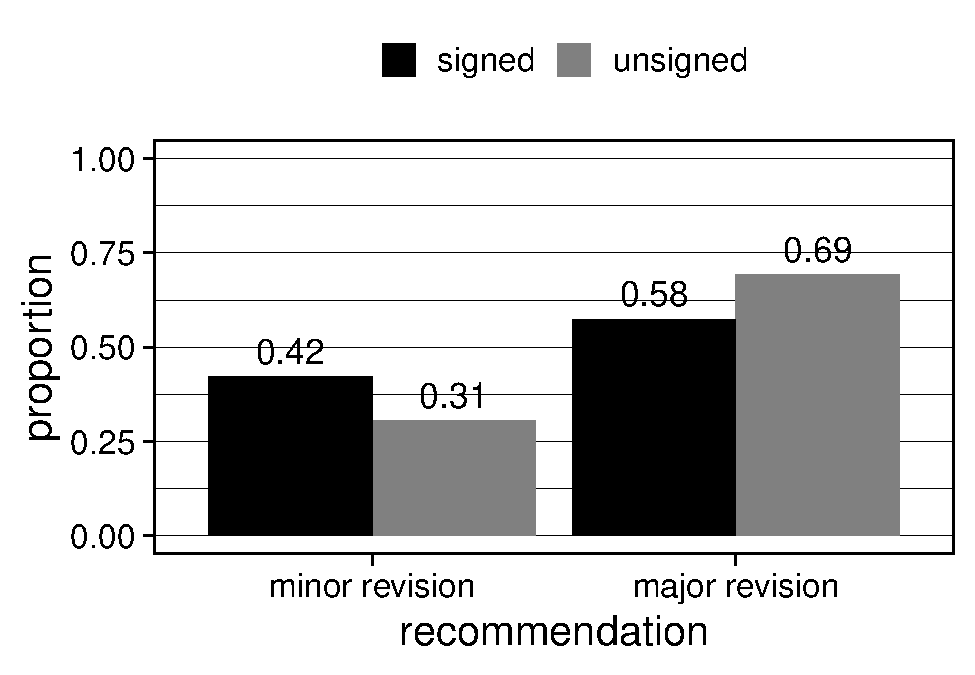
\includegraphics{open_peer_review_files/figure-latex/PeerJrec-1.pdf}
\caption{\label{fig:PeerJrec}Proportion of \enquote{minor revisions} or \enquote{major revisions} recommendations by the handling editor at PeerJ conditioned on whether reviews were signed or unsigned.}
\end{figure}

Analyzing the reviews at the Royal Society provides a more direct answer to our question, since each individual reviewer is asked to provide a recommendation of \enquote{accept}, \enquote{minor revisions}, \enquote{major revisions}, or \enquote{reject}. We can therefore directly compare how recommendations are related to the decision to sign reviews (see Figure \ref{fig:TRSrec}). The overall pattern clearly shows that the proportion of signed reviews is larger for more positive recommendations (accept and minor revisions) whereas the proportion of unsigned reviews is larger for more negative reviews (major revisions and reject).

\begin{figure}
\centering
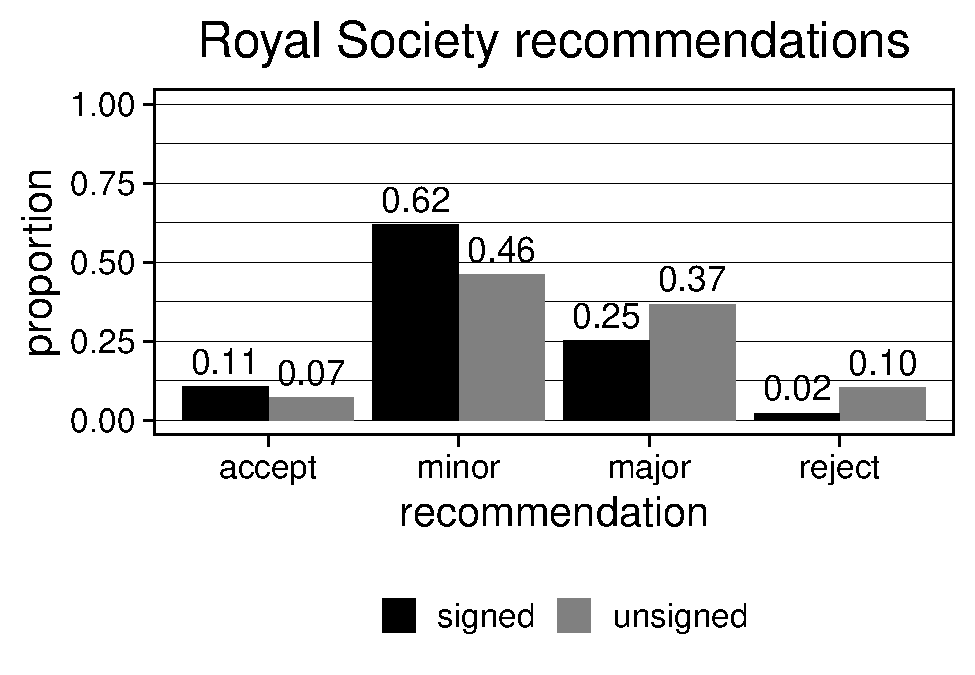
\includegraphics{open_peer_review_files/figure-latex/TRSrec-1.pdf}
\caption{\label{fig:TRSrec}Proportion of \enquote{accept}, \enquote{minor revisions}, \enquote{major revisions}, or \enquote{reject} recommendations by reviewers of Royal Society Open journals conditioned on whether reviews were signed or unsigned.}
\end{figure}

We cannot draw causal conclusions based on this correlational data. It is possible that reviewers are less likely to sign more negative reviews. It is also possible that people who sign their reviews generally give more positive recommendations, and therefore the distribution of signed reviews differs from non-signed reviews. These are just two of many possible explanations for the observed pattern. Based on the literature reviewed in the introduction we know researchers are hesitant to voice criticism when their identity will be known, and experimental evidence suggests that if identities are shared with authors, recommendations become somewhat more positive. Therefore, it seems plausible that at least part of the pattern we observed can be explained by reviewers being more likely to sign more positive reviews. Although we had access to few \enquote{reject} recommendations because we could only access reviews for published manuscripts, the difference between signed and unsigned reviews for major revisions, minor revisions, and accept recommendations replicates the findings by Bravo et al. (2019) across a larger range of research fields, based on a larger dataset, and in journals where a larger percentage of reviewers volunteer to disclose their identity. This replication suggests that the difference in recommendations depending on whether reviews are signed or not is a rather reliable observation.

\onecolumn

\begin{figure}
\centering
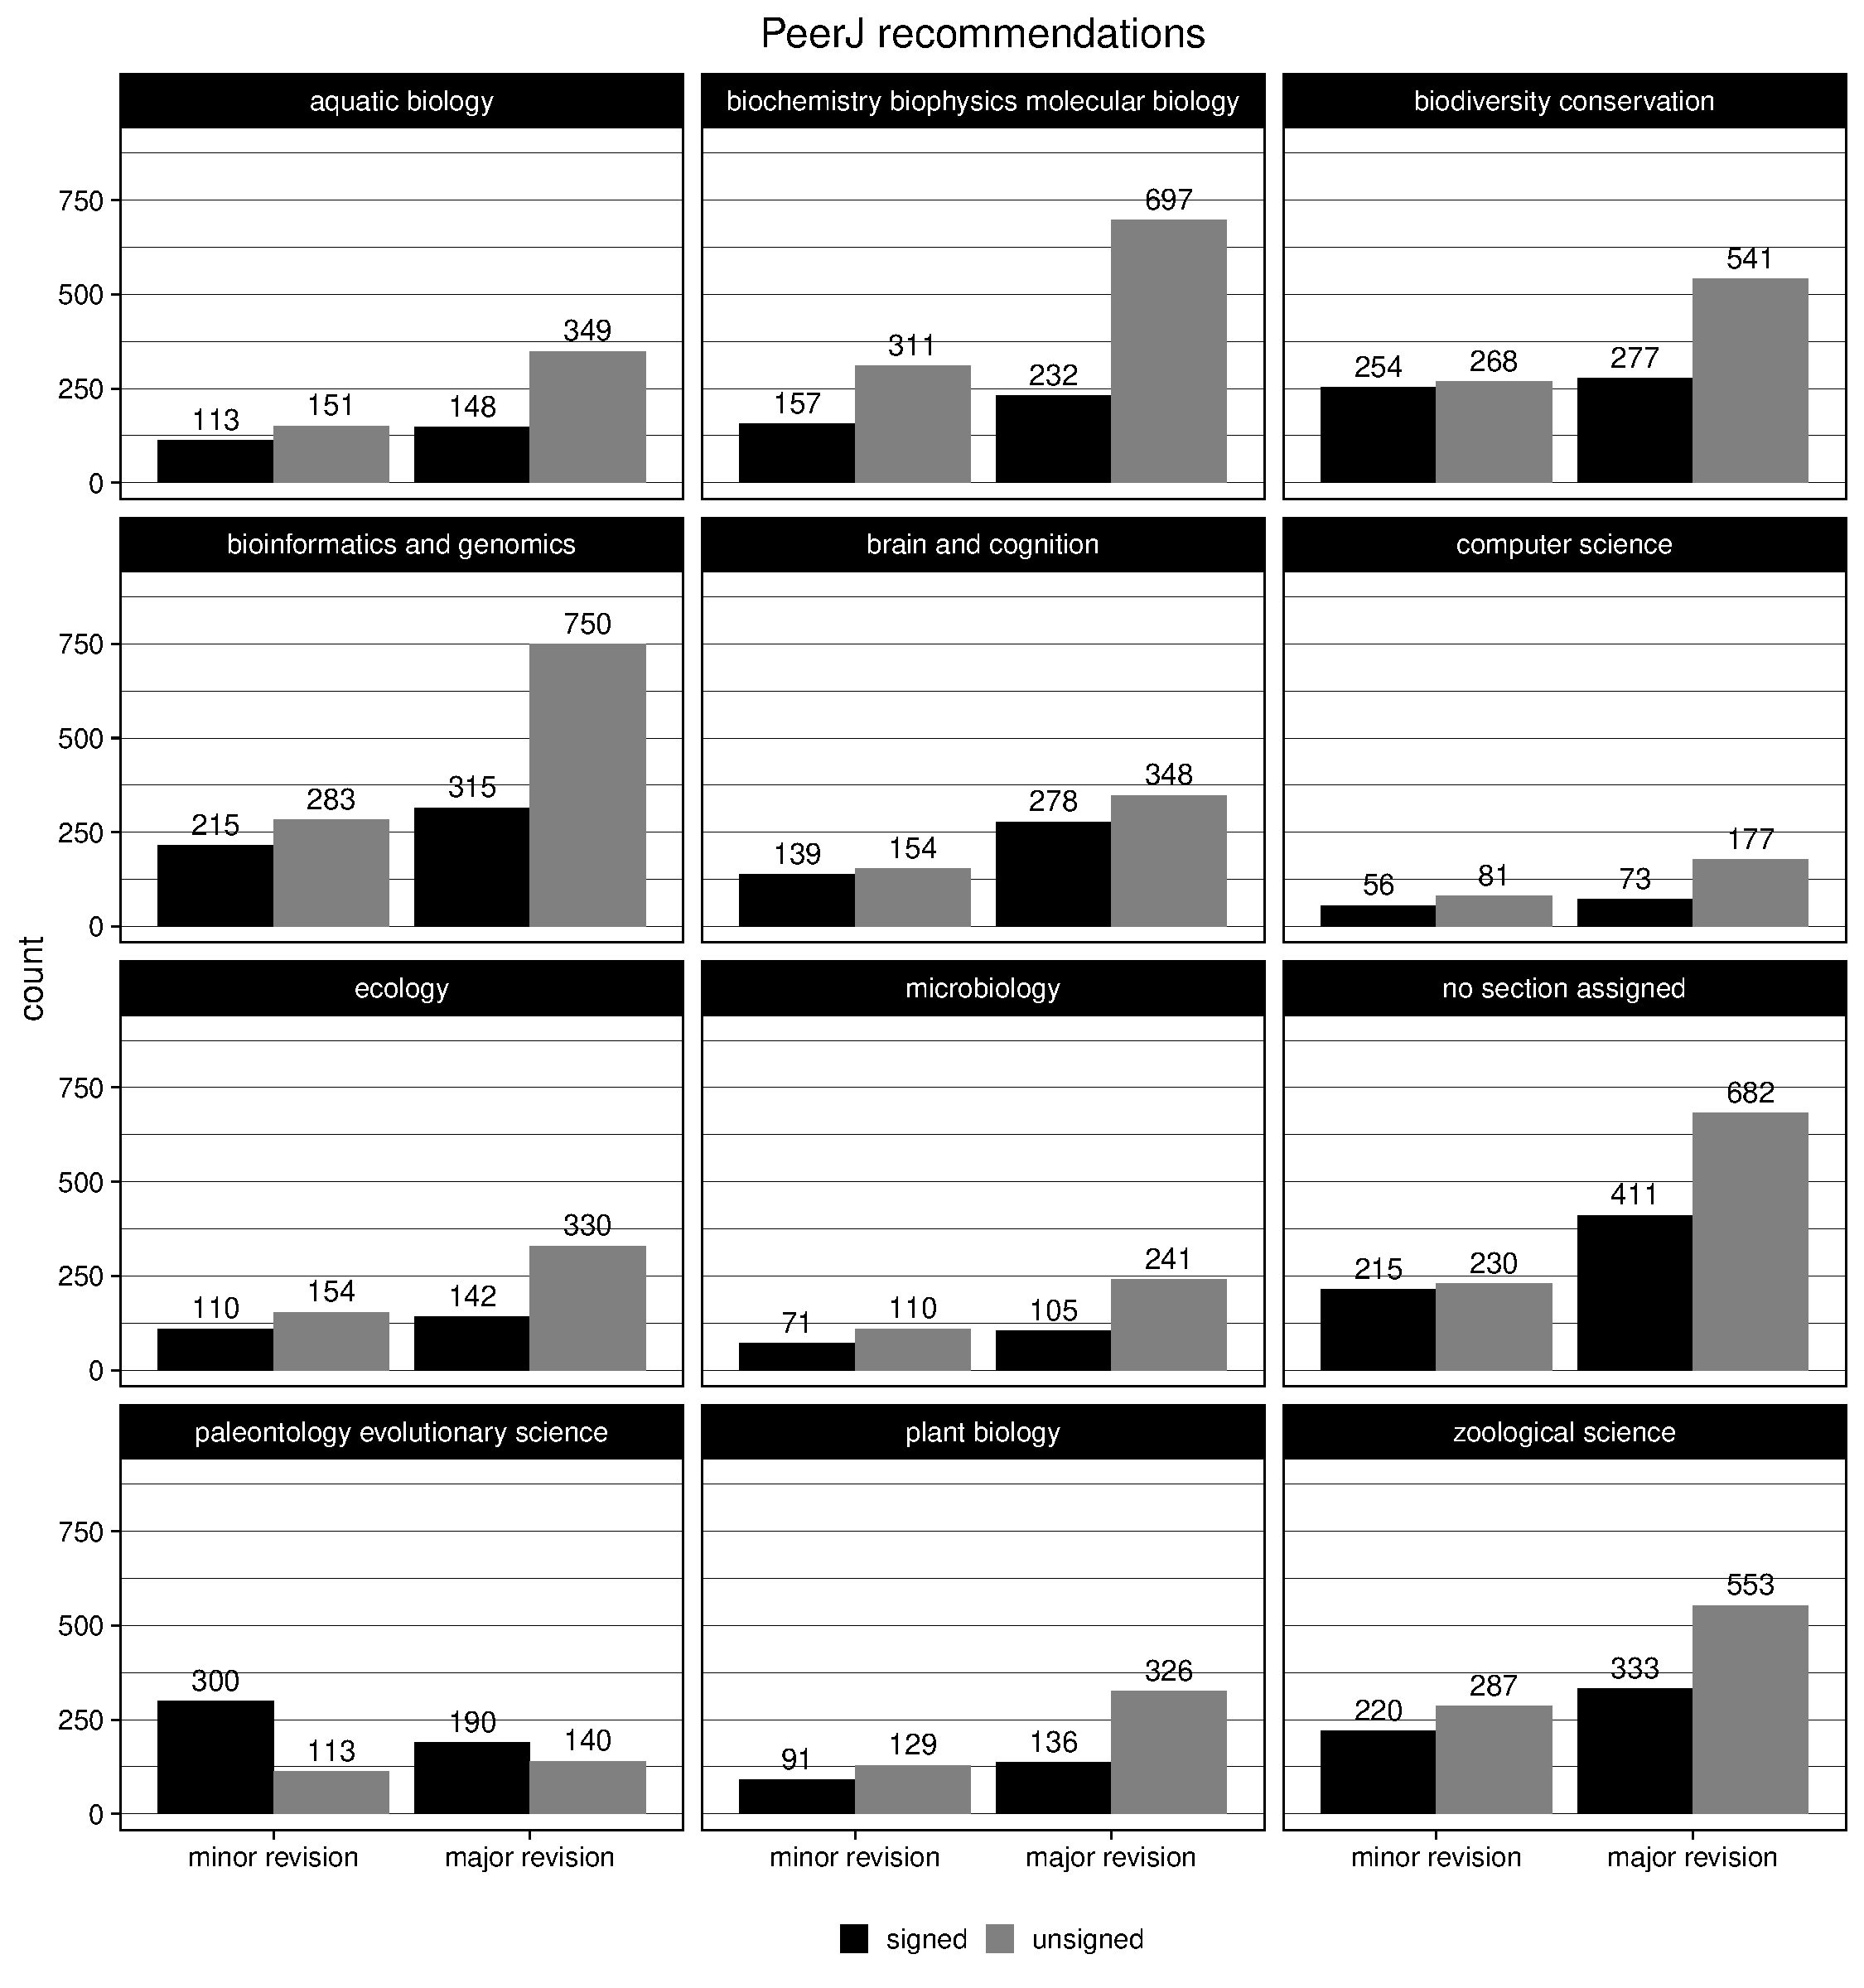
\includegraphics{open_peer_review_files/figure-latex/PeerJrecperfield-1.pdf}
\caption{\label{fig:PeerJrecperfield}Proportion of \enquote{minor revisions} or \enquote{major revisions} recommendations by the handling editor at PeerJ conditioned on whether reviews were signed or unsigned.}
\end{figure}

\begin{figure}
\centering
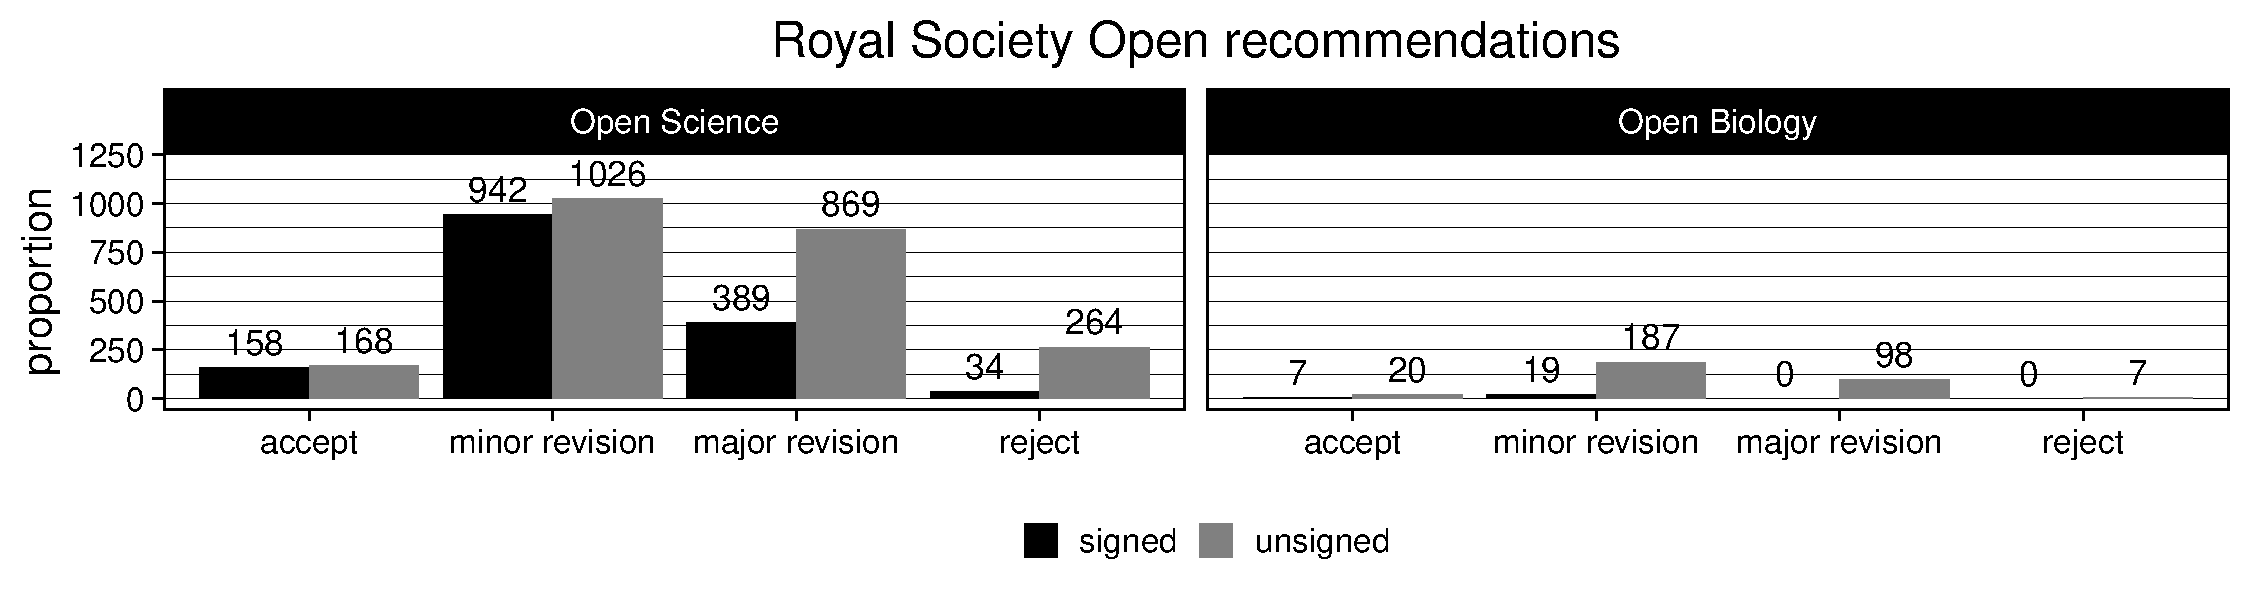
\includegraphics{open_peer_review_files/figure-latex/TRSrecpergroup-1.pdf}
\caption{\label{fig:TRSrecpergroup}Proportion of \enquote{accept}, \enquote{minor revisions}, \enquote{major revisions}, or \enquote{reject} recommendations by reviewers of Royal Society Open journals conditioned on whether reviews were signed or unsigned.}
\end{figure}

\twocolumn

\hypertarget{additional-analyses}{%
\section{Additional Analyses}\label{additional-analyses}}

The dataset we are sharing has information about the recommendations of reviewers (RSOS and RSOB) or editors (PeerJ) after each round of peer review, the names of reviewers who signed their review, and the time in review (114 days for PeerJ, 132 days for Royal Society Open journals). Using the DOI, researchers can link this data to other sources of information such as citation counts. Because the reviews themselves are included in our dataset, researchers can use the text files to answer more detailed questions about the content of peer reviews across different domains. Since we know the individual recommendation of each reviewer for Royal Society Open journals, one example of the insights that open reviews provide is how often reviewers agree. For the 0 papers where the reviews were published, all reviewers agreed on the recommendation for NA articles (NA\% of the time). For NA\% of the manuscripts the maximum deviation was one category (e.g., minor and major revisions), for NA\% of the manuscripts the maximum deviation was two categories (e.g., accept and major revision), and for NA\% of the manuscripts the maximum deviation was three categories (i.e., accept and reject). There were 3 articles where researchers received all four possible recommendations (accept, minor revisions, major revisions, reject) from at least four different reviewers.

Regrettably, neither PeerJ nor Royal Society Open journals make peer reviews available for manuscripts that were rejected. As a consequence, we have analyzed a biased sample of the literature. Few scientific journals make peer reviews available for all submitted articles (for notable exceptions, see Meta-Psychology and F1000). Although open reviews enable us to look in more detail at the peer review process, it would be extremely interesting to be able to follow manuscripts through the peer review process even when they are rejected at one specific journal. Despite this limitation, the pattern of results we observe is very similar to that reported by Bravo et al. (2019) who had access to the reviews for accepted and rejected manuscripts.

\hypertarget{discussion}{%
\section{Discussion}\label{discussion}}

Our analysis shows that when authors are given the choice to sign their reviews, signed reviews have more positive recommendations than unsigned reviews. This pattern is clearly present for reviews in Royal Society Open Science and Open Biology, a large multi-disciplinary journal that publishes articles across a wide range of scientific domains. The pattern is also visible in a second large multi-disciplinary journal, PeerJ, under the assumption that recommendations by editors at PeerJ are correlated with the recommendations by reviewers. Our results replicate and extend earlier findings by Bravo et al. (2019), and complement self-report and experimental results in the literature.

Peer review is generally seen as an important quality control mechanism in science, yet researchers can rarely evaluate the quality of peer review at journals. Open reviews allow researchers to examine meta-scientific questions that give insights into the peer review process. Our data supports the idea that reviewers' decisions to sign are related to their recommendation across a wide range of scientific disciplines. Together with self-report data and experiments reported in the literature, our data increase the plausibility that in real peer reviews at least some reviewers are more likely to sign if their recommendation is more positive. This type of strategic behavior also follows from a purely rational goal to optimize the benefits of peer review while minimizing the costs. For positive recommendations, reviewers will get credit for their reviews, while for negative reviews they do not run the risk of receiving any backlash from colleagues in their field.

It is worthwhile to examine whether this fear of retaliation has an empirical basis, and if so, to consider developing guidelines to counteract such retaliation (Bastian, 2018). Based on all available research it seems plausible that at least some reviewers hesitate to sign if they believe doing so could have negative consequences, but will sign reviews with more positive recommendations to get credit for their work. Therefore, it seems worthwhile to explore ways in which reviewers could be enabled to feel comfortable to claim credit for all their reviews, regardless of whether their recommendation is positive or negative.

\hypertarget{author-contributions}{%
\section{Author Contributions}\label{author-contributions}}

N. van Sambeek and D. Lakens developed the idea, and jointly created the R code to generate and analyze the data. N. van Sambeek drafted the initial version of the manuscript as a Bachelor's thesis, D. Lakens drafted the final version, and both authors revised the final version of the manuscript.

\hypertarget{competing-interests}{%
\section{Competing interests}\label{competing-interests}}

The authors report no conflicts of interest.

\hypertarget{references}{%
\section{References}\label{references}}

\setlength{\parindent}{-0.5in}
\setlength{\leftskip}{0.5in}

\hypertarget{refs}{}
\leavevmode\hypertarget{ref-bastian_signing_2018}{}%
Bastian, H. (2018). Signing Critical Peer Reviews \& the Fear of Retaliation: What Should We Do? \textbar{} Absolutely Maybe. https://blogs.plos.org/absolutely-maybe/2018/03/22/signing-critical-peer-reviews-the-fear-of-retaliation-what-should-we-do/.

\leavevmode\hypertarget{ref-bravo_effect_2019}{}%
Bravo, G., Grimaldo, F., López-Iñesta, E., Mehmani, B., \& Squazzoni, F. (2019). The effect of publishing peer review reports on referee behavior in five scholarly journals. \emph{Nature Communications}, \emph{10}(1), 1--8. \url{https://doi.org/10.1038/s41467-018-08250-2}

\leavevmode\hypertarget{ref-bruce_impact_2016}{}%
Bruce, R., Chauvin, A., Trinquart, L., Ravaud, P., \& Boutron, I. (2016). Impact of interventions to improve the quality of peer review of biomedical journals: A systematic review and meta-analysis. \emph{BMC Medicine}, \emph{14}. \url{https://doi.org/10.1186/s12916-016-0631-5}

\leavevmode\hypertarget{ref-godlee_making_2002}{}%
Godlee, F. (2002). Making Reviewers Visible: Openness, Accountability, and Credit. \emph{JAMA}, \emph{287}(21), 2762--2765. \url{https://doi.org/10.1001/jama.287.21.2762}

\leavevmode\hypertarget{ref-mulligan_peer_2013}{}%
Mulligan, A., Hall, L., \& Raphael, E. (2013). Peer review in a changing world: An international study measuring the attitudes of researchers. \emph{Journal of the American Society for Information Science and Technology}, \emph{64}(1), 132--161. \url{https://doi.org/10.1002/asi.22798}

\leavevmode\hypertarget{ref-ooms_pdftools_2019}{}%
Ooms, J. (2019). \emph{Pdftools: Text extraction, rendering and converting of PDF documents}.

\leavevmode\hypertarget{ref-r_core_team_r_2013}{}%
R Core Team. (2013). \emph{R: A language and environment for statistical computing}. Vienna, Austria: R Foundation for Statistical Computing.

\leavevmode\hypertarget{ref-ross-hellauer_survey_2017}{}%
Ross-Hellauer, T., Deppe, A., \& Schmidt, B. (2017). Survey on open peer review: Attitudes and experience amongst editors, authors and reviewers. \emph{PLOS ONE}, \emph{12}(12), e0189311. \url{https://doi.org/10.1371/journal.pone.0189311}

\leavevmode\hypertarget{ref-spellman_short_2015}{}%
Spellman, B. A. (2015). A Short (Personal) Future History of Revolution 2.0. \emph{Perspectives on Psychological Science}, \emph{10}(6), 886--899. \url{https://doi.org/10.1177/1745691615609918}

\leavevmode\hypertarget{ref-walsh_open_2000}{}%
Walsh, E., Rooney, M., Appleby, L., \& Wilkinson, G. (2000). Open peer review: A randomised controlled trial. \emph{The British Journal of Psychiatry}, \emph{176}(1), 47--51. \url{https://doi.org/10.1192/bjp.176.1.47}

\leavevmode\hypertarget{ref-wang_open_2016}{}%
Wang, P., You, S., Manasa, R., \& Wolfram, D. (2016). Open peer review in scientific publishing: A Web mining study of PeerJ authors and reviewers. \emph{Journal of Data and Information Science}, \emph{1}(4), 60--80.

\leavevmode\hypertarget{ref-wickham_stringr_2019}{}%
Wickham, H. (2019). \emph{Stringr: Simple, consistent wrappers for common string operations}.

\end{document}
